% ============================================== %
% Author:Lucian Dorin Crainic <https://luciancrainic.github.io/>
%
% Data Analysis e Visualization of the movements of patients with Fear of Falling.
% 
% Bachelor of Science in Computer Science Thesis, Sapienza University of Rome.
%
% https://github.com/LucianCrainic/Thesis/
%
% ============================================== %

% Document Class
\documentclass[binding=0.6cm]{sapthesis}

% Packages
\usepackage{microtype}
\usepackage[english]{babel}
\usepackage[utf8]{inputenc}
\usepackage[hidelinks]{hyperref}
\usepackage{listings}
\usepackage{xcolor}
\usepackage{geometry} 
\usepackage{caption}  
\usepackage{float}    
\usepackage{lipsum}  
\usepackage{xargs}                     

\usepackage[colorinlistoftodos,prependcaption,textsize=tiny]{todonotes}
\newcommandx{\unsure}[2][1=]{\todo[linecolor=red,backgroundcolor=red!25,bordercolor=red,#1]{#2}}
\newcommandx{\change}[2][1=]{\todo[linecolor=blue,backgroundcolor=blue!25,bordercolor=blue,#1]{#2}}
\newcommandx{\info}[2][1=]{\todo[linecolor=OliveGreen,backgroundcolor=OliveGreen!25,bordercolor=OliveGreen,#1]{#2}}
\newcommandx{\improvement}[2][1=]{\todo[linecolor=Plum,backgroundcolor=Plum!25,bordercolor=Plum,#1]{#2}}
\newcommandx{\thiswillnotshow}[2][1=]{\todo[disable,#1]{#2}}


% Settings
\definecolor{codegreen}{rgb}{0,0.6,0}
\definecolor{blue}{rgb}{0.01, 0.28, 1.0}
\definecolor{codegray}{rgb}{0.5,0.5,0.5}
\definecolor{codepurple}{rgb}{0.58,0,0.82}
\definecolor{backcolour}{rgb}{0.95,0.95,0.92}
\lstdefinestyle{mystyle}{
    backgroundcolor=\color{white},   
    commentstyle=\color{codegreen},
    keywordstyle=\bfseries \color{blue},
    numberstyle=\color{codegray},
    stringstyle=\color{codepurple},
    basicstyle=\footnotesize,
    breakatwhitespace=false,         
    breaklines=true,                 
    captionpos=b,                    
    keepspaces=true,                 
    numbers=left,                    
    numbersep=5pt,                  
    showspaces=false,                
    showstringspaces=false,
    showtabs=false,                  
    tabsize=2
}
\lstset{style=mystyle}

% Metadata
\hypersetup{pdftitle={Thesis},pdfauthor={Lucian Dorin Crainic}}
\title{A Comparative Study of Machine Learning Models for Kinect Skeleton Data in Movement Classification}
\author{Lucian Dorin Crainic}
\IDnumber{1938430}
\course{Bachelor's Degree in Computer Science}
\courseorganizer{Faculty of Information Engineering, Computer Science and Statistics}
\AcademicYear{2023/2024}
\advisor{Prof. Maurizio Mancini}
\authoremail{crainic.lucian@gmail.com}
\copyyear{2022}
\thesistype{Bachelor's Thesis}

% ================== DOCUMENT ==================
\begin{document}

\lstset{language=Python}

\frontmatter

\maketitle

% ================== DEDICATION ==================
% \dedication{
%     It does not matter how slowly you go as long as you do not stop.\\ \emph{Confucius} 
% }

% ================== ABSTRACT ==================
%\begin{abstract}
    This thesis conducts a detailed comparative study of several Machine Learning models, with a focus on their application to Kinect skeleton data for classifying human movements. The primary aim of this research is to evaluate these models to determine the most effective ones for accurately classifying movements recorded through Kinect sensors.\\

    This study begins with an introduction to Kinect technology, highlighting its ability to capture detailed movement data. Following this, an examination of a range of Machine Learning models, such as Support-Vector Machines, Random Forests, Linear Regression and so on. Each model is tested to evaluate its accuracy, processing efficiency and robustness in accurately classifying various movements. 
    
    The core of this comparative analysis is a diverse dataset consisting of several movements captured through a Microsoft Kinect. The research methodology involves several steps: processing the data, extracting key features that are characteristic of specific movements, and applying the selected models to this improved data. Performance evaluation of each model using standard metrics like accuracy, precision, recall and F1 score, which provide a complete picture of their effectiveness. \\
    
    Over this study, valuable understandings are gained into the specific strengths and limitations of each model in the context of movement classification. The findings reveal that some models prove enhanced performance in certain situations, which is influenced by factors like the complexity of the captured movements and the characteristics of the dataset. 
    
    This thesis acts as a useful guide for researchers and professionals. It helps them pick the best models for similar work and sets the stage for more research in this area. The findings can be used to develop more accurate and efficient models for classifying human movements.
\end{abstract}

\let\cleardoublepage\clearpage


\cleardoublepage

\tableofcontents
\let\cleardoublepage\clearpage

\mainmatter

% ================== CHAPTER 1 ==================
% ============================================== %
%
% TODO: 
%
%% ============================================== %
\chapter{Introduction}

   % add todo notes
   
   % \todo[inline]{Add a description of the thesis structure. This is a good place to start to explain briefly every chapter. Do this after you have written the rest of the thesis.}
   
   \section{Problem Statement}

   \section{Literature Review}
   
   \section{Dataset Overview}
   % In this study, we utilized a Kinect Skeleton dataset, provided by the PsyComp Lab.,which plays a crucial role in the development of this research. This dataset is composed of recorded movements performed by a group of 22 individuals. The movements were performed in front of a Kinect sensor, which recorded the movements and saved them as a series of 3D coordinates. The dataset contains 10 different movements, each performed a various number of times by each individual. The movements are as follows:

%    \begin{table}[ht]
%       \centering
%       \begin{tabular}{@{}ccc@{}}
%           \toprule
%           \textbf{No.} & \textbf{Movement Name} & \textbf{Description} \\
%           \midrule
%           1 & \textit{Reach Overhead} & \begin{tabular}[t]{@{}p{9cm}@{}} In a standing position, the subject raises one of their arms above their head.\end{tabular} \\
          
%           2 & \textit {Chair to Chair} & \begin{tabular}[t]{@{}p{9cm}@{}} Starting from a sitting position, the subject stands up, then sits down on another chair.\end{tabular} \\
          
%           3 & \textit{Cross-Reach Left} & \begin{tabular}[t]{@{}p{9cm}@{}} In a standing position, the subject using their left arm reaches across their body to the right side.\end{tabular} \\
          
%           4 & \textit{Cross-Reach Right} & \begin{tabular}[t]{@{}p{9cm}@{}} Description 4 \end{tabular} \\
          
%           5 & \textit{Reach Forward} & \begin{tabular}[t]{@{}p{9cm}@{}} Description 5 \end{tabular} \\
          
%           6 & \textit{Hoop Walk} & \begin{tabular}[t]{@{}p{9cm}@{}} Description 6 \end{tabular} \\
          
%           7 & \textit{Right Leg Stand} & \begin{tabular}[t]{@{}p{9cm}@{}} Description 7 \end{tabular} \\
          
%           8 & \textit{Left Leg Stand} & \begin{tabular}[t]{@{}p{9cm}@{}} Description 8 \end{tabular} \\
          
%           9 & \textit{Mat Walk} & \begin{tabular}[t]{@{}p{9cm}@{}} Description 9 \end{tabular} \\
          
%           10 & \textit{TUG Walk} & \begin{tabular}[t]{@{}p{9cm}@{}} The Timed Up and Go Walk, a common test used to assess mobility and fall risk in elderly individuals.\end{tabular} \\
%           \bottomrule
%       \end{tabular}
%       \caption{Movements used in this study, along with a brief description.}
%       \label{tab:movement_table}
%   \end{table}

   \section{Aims and Objectives of the Study} 
   
   % \begin{enumerate}
   %    \item \textbf{Kinect Data Processing}: Process Kinect Skeleton Data from elderly individuals performing ten specific movements as part of the Fear of Falling assessment.
   %    \item TODO {}
   %    \item TODO
   %    \item TODO
   % \end{enumerate}

\cleardoublepage

% ================== CHAPTER 2 ==================
\chapter{Literature Review}
    \section{Fear of falling: definition and prevalence}
    \section{Factors contributing to fear of falling}
    \section{Consequences of fear of falling}

% ================== CHAPTER 3 ==================
% ============================================== %
%
% TODO: 
%
%% ============================================== %
\chapter{Methodology}
    \section{Overview of Models Analyzed}
        \subsection{Scikit-Learn}  
        \subsection{Models Selection}
    \section{Selected Models for In-Depth Examination}
        \subsection{Support Vector Machine}
        \subsection{Random Forest}
        \subsection{Gradient Boosting}
        \subsection{Logistic Regression}
        \subsection{Linear Discriminant Analysis}
        \subsection{Multi-layer Perceptron}
    \section{Data Splitting Methods}
        \subsection{Ineffective Approach}
        \subsection{Effective Approach}
        \subsection{Sequential Data Approach}
    \section{Feature Engineering}
        \subsection{Feature Selection}

\cleardoublepage

% ================== CHAPTER 4 ==================
\hypersetup{colorlinks=true, linkcolor=blue, citecolor=red}

\chapter{Results and Discussion} \label{chap:results_and_discussion}

    This chapter presents results obtained from experiments conducted in the previous chapter. Classification models are evaluated using different approaches and metrics. Results are then discussed and compared to each other.

    \section{Models evaluation}

        Performed using \textit{Scikit-Learn} library \cite{sklearn_api}. It provides a wide range of validation methods and metrics to evaluate the performance of the models. The following sections will present validation methods and metrics used in this thesis.

        \subsection{Validation}

            Validation is a process of evaluating the performance of the models. The goal of validation is to estimate the performance of the model on new data, not used during the training process. The following validation methods are used:

            \subsubsection{Hold-Out}

                This method is widely used for its simplicity and speed. The dataset is split into two subsets. The training set is used to train the model, Testing set is used to evaluate the performance of the model. Typically, a common split ratio is:
                \begin{itemize}
                    \item \textbf{Training set}: 70\% of the dataset.
                    \item \textbf{Testing set}: 30\% of the dataset.
                \end{itemize}
            
            \subsubsection{Cross-Validation}
                
                This method is used in literature for its effectiveness and robustness. It can be time-consuming for large datasets, but it is the best method to evaluate the performance of the models.

                \begin{itemize}

                    \item \textbf{K fold}: Data is divided into \textit{K} folds, then \textit{K-1} folds are used for training, and the remaining fold is used for testing. This process is repeated \textit{K} times, with each fold being used exactly once for testing. Fig \ref{fig:kfold} display KFold split.
                    
                    \begin{figure}[H]
                        \centering
                        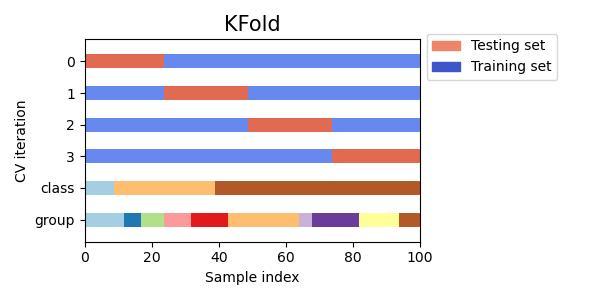
\includegraphics[width=1.0\textwidth]{../src/resources/images/other/kfold.png}
                        \caption{
                          KFold Visualization from Scikit-Learn documentation \cite{scikit-learn}.
                        }
                        \label{fig:kfold}
                    \end{figure}

                    \item \textbf{Group k fold}: Variation of k fold designed for situations where data has inherent groupings or dependencies that should be preserved in train/test split. In this method, data is divided into \textit{K} folds, and then an additional constraint is imposed to ensure that data points from the same group are in the same fold. Fig \ref{fig:groupkfold} display GroupKFold split.
                    
                    \begin{figure}[H]
                        \centering
                        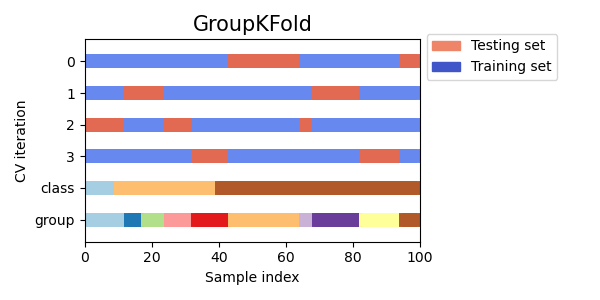
\includegraphics[width=1.0\textwidth]{../src/resources/images/other/groupkfold.png}
                        \caption{
                          GroupKFold Visualization from Scikit-Learn documentation \cite{scikit-learn}.
                        }
                        \label{fig:groupkfold}
                    \end{figure}
                \end{itemize}
                
        An advantage of using \textit{Cross-Validation} over \textit{Hold-Out} is that all samples are used for both training and testing, and each sample is used for testing exactly once. This method helps to reduce the variance of the estimated performance of a model, by averaging results over several trials. A disadvantage of using Cross-Validation is that it is computationally expensive for very large datasets. \\ 

        In this thesis, both methods are used to evaluate the performance of the models. The Hold-Out method is used to evaluate the performance of the models for \textit{Wrong approach} and \textit{Sequence approach} datasets due to their large dimensions. Cross-Validation method is used with the Hold-Out method to evaluate the performance of the models for \textit{Correct approach} and \textit{Feature Engineering approach} dataset due to them scoring the best results and being effective approaches. Confronting the results of two methods will show the correctness of an evaluation. \\
        
        \subsection{Metrics}

            This section will report metrics used to benchmark different models used in this thesis.

            \subsubsection{Accuracy score}

                \textit{Accuracy} is a proportion of correct predictions, considering both true positives and true negatives, among a total number of samples. The formula used to calculate accuracy is the following:
                \begin{equation}
                    \frac{\text{TP} + \text{TN}}{\text{TP} + \text{TN} + \text{FP} + \text{FN}}
                \end{equation} 
                where \textbf{TP} is a number of true positives, \textbf{TN} is a number of true negatives, \textbf{FP} is a number of false positives and \textbf{FN} is a number of false negatives.

            \subsubsection{Precision score}

                \textit{Precision} is the ability of a classifier not to label as positive a sample that is negative. The formula used to calculate precision is the following:
                \begin{equation}
                    \frac{\text{TP}}{\text{TP} + \text{FP}}
                \end{equation}

            \subsubsection{Recall score}

                \textit{Recall} is the ability of a classifier to find all the positive samples. The formula used to calculate the recall is the following:
                \begin{equation}
                    \frac{\text{TP}}{\text{TP} + \text{FN}}
                \end{equation}

            \subsubsection{F1 score}

                \textit{F1 score} is a harmonic mean of precision and recall. The formula used to calculate the F1 score is the following:
                \begin{equation}
                    \frac{ 2 \times (\text{precision} \times \text{recall})}{\text{precision} + \text{recall}}
                \end{equation}

            \subsubsection{Matthews correlation coefficent} 

                \textit{Matthews correlation coefficent} (or $\varphi$ coefficient) takes into account true and false positives and negatives and is regarded as a balanced measure that can be used even if the classes are of very different sizes. Formula used to calculate $\varphi$ coefficient is as follows: 
                \begin{equation}
                    \frac{\text{TP} \times \text{TN} - \text{FP} \times \text{FN}}{\sqrt{(\text{TP} + \text{FP})(\text{TP} + \text{FN})(\text{TN} + \text{FP})(\text{TN} + \text{FN})}}
                \end{equation}

            These metrics will be used to show the effectiveness of the approaches proposed in this thesis.
    
\section{Results}
        
        Combining validation methods and metrics presented above, the following tables will show results obtained from experiments conducted. Results are divided into two categories: \textbf{Exploratory} shows two approaches that were tested but did not obtain good results due to wrong implementation or loss of information. \textbf{Effective} shows two approaches that obtained good results and are suitable for this task. Presented in the following order: \textit{Traditional approach}, \textit{Sequence approach}, \textit{Effective approach} and \textit{Feature Engineering approach}. 

        \subsection{Exploratory}

            The following approaches are included because they are a starting point in this thesis, and show how different implementations can affect the accuracy of the models.
            
            \subsubsection{Traditional approach}
                
                Presented in Section \ref{sec:badsplit}, it is the first one to be tested and it got surprisingly good results. Such a simple approach and yet high accuracy raised doubts about the validity of results, after further investigation, it has been discovered that the dataset is not properly split into training and testing sets. 
            
                \begin{table}[htbp]
                    \centering
                    \begin{tabular}{lrrrrr}
                        \toprule
                        \textbf{Model} & \textbf{Accuracy} & \textbf{F1} & \textbf{Recall} & \textbf{Precision} & \textbf{MCC} \\
                        \midrule
                        Random Forests & \textbf{0.99} & \textbf{0.99} & \textbf{0.99} & \textbf{0.99} & \textbf{0.99} \\
                        K-Nearest Neighbors & 0.98 & 0.98 & 0.98 & 0.98 & 0.98 \\
                        Decision Trees & 0.96 & 0.96 & 0.96 & 0.96 & 0.96 \\
                        Support-Vector Machines & 0.87 & 0.86 & 0.85 & 0.86 & 0.86 \\
                        Logistic Regression & 0.82 & 0.80 & 0.80 & 0.80 & 0.80 \\
                        \bottomrule
                    \end{tabular}
                    \caption{Evaluation results using \textbf{Hold-Out} validation method.}
                    \label{tab:wrong_approach_holdout}
                \end{table}

                In Table \ref{tab:wrong_approach_holdout}, results obtained from the Hold-Out method are presented. High values are obtained for all the metrics, with \textbf{Random Forests} obtaining the highest values with a score of \textbf{0.99} for accuracy. This confirmed doubts about the validity of results, a patient is both present in the training and testing set. This led to models \textbf{overfitting} the data and obtaining high accuracy.

            \subsubsection{Sequence approach}

                Presented in Section \ref{sec:seqsplit}, it achieved the lowest results of all the approaches. Tested to see if concatenating frames of a movement into a sequence would help models differentiate between movements and obtain higher accuracy. 
                
                \begin{table}[htbp]
                    \centering
                    \begin{tabular}{lrrrrr}
                        \toprule
                        \textbf{Model} & \textbf{Accuracy} & \textbf{F1} & \textbf{Recall} & \textbf{Precision} & \textbf{MCC} \\
                        \midrule
                        K-Nearest Neighbors & \textbf{0.56} & \textbf{0.54} & \textbf{0.54} & \textbf{0.54} & \textbf{0.51} \\
                        Random Forests & 0.55 & 0.52 & 0.53 & 0.53 & 0.49 \\
                        Support-Vector Machines& 0.52 & 0.47 & 0.49 & 0.46 & 0.47 \\
                        Logistic Regression & 0.44 & 0.41 & 0.42 & 0.43 & 0.38 \\
                        Decision Trees & 0.41 & 0.38 & 0.39 & 0.40 & 0.34 \\
                        \bottomrule
                    \end{tabular}
                    \caption{Evaluation results using \textbf{Hold-Out} validation method.}
                    \label{tab:sequence_approach_holdout}
                \end{table}

                In Table \ref{tab:sequence_approach_holdout}, results obtained from the Hold-Out method are presented. Low values are obtained for all the metrics, with \textbf{K-Nearest Neighbor} obtaining the highest values with a score of \textbf{0.56} for accuracy. These results are considered low based on other approaches, however in the context of randomly guessing a movement of a patient accuracy would be \textbf{0.10} as there are 10 movements. This means that models can differentiate between movements, but sequence implementation leads to a loss of information and a high accuracy cannot be obtained.

        \subsection{Effective}

                The following approaches obtained the best results and are suitable for this task. The main difference between the two approaches is in the data used to train the models. \textit{Correct Approach} uses data as it is from the Kinect sensor, while \textit{Feature Engineering Approach} uses data after applying Feature Engineering techniques.
                
            \subsubsection{Correct approach}

                Presented in Section \ref{sec:goodsplit}, considered effective because raw Kinect data can obtain a high accuracy. Data is not modified in any way, besides the removal of rotational and state data, and pre-processing to remove noise.\\
                 
                In Table \ref{tab:correct_approach_holdout} results obtained from the Hold-Out method are presented. \textbf{Random Forests} obtains the highest values for all the metrics, with a score of \textbf{0.74} for accuracy. Other models such as \textit{Gradient Boosting}, \textit{Linear Discriminant Analysis}, \textit{Support-Vector Machines}, \textit{K-Nearest Neighbors} obtained great results as well with a score greater than \textbf{0.70} for accuracy. This confirms that data obtained from the Kinect sensor is suitable for the task of movement classification without any major tweaks.\\
                
                \newpage

                \begin{table}[htbp]
                    \centering
                    \begin{tabular}{lrrrrr}
                        \toprule
                        \textbf{Model} & \textbf{Accuracy} & \textbf{F1} & \textbf{Recall} & \textbf{Precision} & \textbf{MCC} \\
                        \midrule
                        Random Forests & \textbf{0.74} & \textbf{0.73} & \textbf{0.73} & \textbf{0.73} & \textbf{0.71} \\
                        Gradient Boosting & 0.73 & 0.72 & 0.72 & 0.72 & 0.69 \\
                        Linear Discriminant Analysis & 0.72 & 0.71 & 0.71 & 0.74 & 0.68 \\
                        Support Vector Machines & 0.71 & 0.71 & 0.71 & 0.72 & 0.68 \\
                        K-Nearest Neighbors & 0.71 & 0.69 & 0.69 & 0.70 & 0.67 \\
                        Logistic Regression & 0.66 & 0.64 & 0.64 & 0.64 & 0.62 \\
                        Multi-Layer Perceptron & 0.63 & 0.59 & 0.62 & 0.61 & 0.59 \\
                        Naive Bayes & 0.63 & 0.60 & 0.61 & 0.62 & 0.58 \\
                        Decision Trees & 0.63 & 0.60 & 0.62 & 0.61 & 0.58 \\
                        Ada Boost & 0.35 & 0.22 & 0.28 & 0.24 & 0.32 \\
                        \bottomrule
                    \end{tabular}
                    \caption{Evaluation results using \textbf{Hold-Out} validation method.}
                    \label{tab:correct_approach_holdout}
                \end{table}

                In Table \ref{tab:correct_approach_holdout} \textbf{Hold-Out} validation method is used for all models, while in Table \ref{tab:correct_approach_cv} \textbf{Cross-Validation} is used with only 3 models to compare two validation methods and show that there is no major difference between them. The results obtained from the two methods are similar. \\

                Hold-Out method is used for its speed, with \textbf{10 minutes} of training time while Cross-Validation runs for hours without finishing. This is because this approach uses raw Kinect data, that contains over \textbf{59000} rows and \textbf{100} columns. 
                
                \begin{table}[htbp]
                    \centering
                    \begin{tabular}{|c|c|c|}
                    \hline
                    \textbf{Model} & \textbf{Cross-Validation} & \textbf{Hold-Out} \\ \hline
                        Linear Discriminant Analysis    & 0.73 & 0.72 \\ 
                                                        & 0.71 & 0.71 \\ 
                                                        & 0.70 & 0.71 \\ 
                                                        & 0.75 & 0.74 \\
                                                        & 0.70 & 0.68 \\ 
                                                        \hline
                        K-Nearest Neighbors             & 0.71 & 0.71 \\ 
                                                        & 0.70 & 0.69 \\ 
                                                        & 0.70 & 0.69 \\ 
                                                        & 0.71 & 0.70 \\
                                                        & 0.68 & 0.67 \\
                                                        \hline
                        Naive Bayes                     & 0.66 & 0.63 \\ 
                                                        & 0.62 & 0.60 \\ 
                                                        & 0.63 & 0.62 \\
                                                        & 0.66 & 0.61 \\ 
                                                        & 0.62 & 0.58 \\ 
                                                        \hline
                    \end{tabular}
                    \caption{Comparison of obtained results with Cross-Validation and Hold-Out methods. Metrics reported are (from top to bottom): Accuracy, F1, Recall, Precision, MCC.}
                    \label{tab:correct_approach_cv}
                \end{table}
                \newpage
                In Table \ref{tab:correct_approach_mat_hoop} are displayed results of a final approach, where two movements \textit{Mat Walk} and \textit{Hoop Walk} are removed from the dataset one at a time. Results show that the accuracy of models increased by \textbf{4\%} to \textbf{5\%}. This is because the two movements are very similar, and this caused models to struggle to differentiate between them no matter the features used. \\
                By removing either one of the movements, the model's accuracy increased by the same amount. This leaves a decision to the user to choose which movement to remove based on the context of the application. 

                \begin{table}[htbp]
                    \centering
                    \begin{tabular}{|c|c|c|}
                    \hline
                    \textbf{Model} & \textbf{Hoop Walk Removed} & \textbf{Mat Walk Removed} \\ \hline
                        Random Forests                   & 0.79 & 0.79 \\ 
                                                        & 0.79 & 0.79 \\ 
                                                        & 0.79 & 0.79 \\ 
                                                        & 0.79 & 0.79 \\
                                                        & 0.76 & 0.76 \\ 
                                                        \hline
                        Gradient Boosting               & 0.78 & 0.78 \\ 
                                                        & 0.78 & 0.78 \\ 
                                                        & 0.78 & 0.78 \\ 
                                                        & 0.78 & 0.79 \\
                                                        & 0.74 & 0.75 \\
                                                        \hline
                        Linear Discriminant Analysis    & 0.76 & 0.76 \\ 
                                                        & 0.77 & 0.77 \\ 
                                                        & 0.76 & 0.76 \\
                                                        & 0.80 & 0.79 \\ 
                                                        & 0.73 & 0.73 \\ 
                                                        \hline
                    \end{tabular}
                    \caption{Comparison of obtained results with Mat Walk and Hoop Walk removed from the dataset. Metrics reported are (from top to bottom): Accuracy, F1, Recall, Precision, MCC.}
                    \label{tab:correct_approach_mat_hoop} 
                \end{table}
           \newpage 

            \subsubsection{Feature engineering approach}
                
                Presented in Section \ref{sec:feature_engineering}, considered most effective because it obtained the highest accuracy of all approaches and it is fastest to train. Data is modified by applying Feature Engineering techniques presented in \ref{sec:feature_engineering}, this leads to the dataset having fewer rows and columns.
            
            \begin{table}[htbp]
                \centering
                \begin{tabular}{lrrrrr}
                    \toprule
                    \textbf{Model} & \textbf{Accuracy} & \textbf{F1} & \textbf{Recall} & \textbf{Precision} & \textbf{MCC} \\
                    \midrule
                    Multi-Layer Perceptron & \textbf{0.83} & \textbf{0.83} & \textbf{0.84} & \textbf{0.84} & \textbf{0.81} \\
                    Logistic Regression & 0.82 & 0.83 & 0.83 & 0.84 & 0.80 \\
                    Linear Discriminant Analysis & 0.81 & 0.82 & 0.83 & 0.84 & 0.80 \\
                    Support-Vector Machines & 0.81 & 0.82 & 0.83 & 0.83 & 0.80 \\
                    Random Forests & 0.79 & 0.80 & 0.80 & 0.82 & 0.77 \\
                    Gradient Boosting & 0.78 & 0.79 & 0.79 & 0.82 & 0.76 \\
                    K-Nearest Neighbors & 0.78 & 0.79 & 0.80 & 0.80 & 0.76 \\
                    Decision Trees & 0.73 & 0.73 & 0.74 & 0.77 & 0.70 \\
                    Naive Bayes & 0.63 & 0.63 & 0.66 & 0.66 & 0.60 \\
                    Ada Boost & 0.46 & 0.38 & 0.46 & 0.42 & 0.43 \\
                    \bottomrule
                \end{tabular}
                \caption{Evaluation results using \textbf{Cross-Validation} method.}
                \label{tab:feature_engineering_approach_cv}
            \end{table}

            In Table \ref{tab:feature_engineering_approach_cv} results obtained from the Cross-Validation method are displayed. High values are obtained for all metrics, with \textbf{Multi-Layer Perceptron}  and \textbf{Logistic Regression} obtaining the highest values with a score of \textbf{0.83} and \textbf{0.82} for accuracy. Other models such as \textit{Linear Discriminant Analysis}, \textit{Gradient Boosting}, \textit{Random Forests}, \textit{Support-Vector Machines}, \textit{K-Nearest Neighbors} obtained great results as well with a score greater than \textbf{0.70} for accuracy. 

            This confirms that Feature Engineering techniques applied to data are suitable for the task of movement classification. This approach is also the fastest to train, with a training time of \textbf{1 minute}. \\

            Table \ref{tab:feature_engineering_approach_holdout} presents results obtained from the Hold-Out validation method. Similar to the ones obtained with the validation method, with a lower training time of \textbf{10 seconds}. However, Cross-Validation is preferred over Hold-Out because it is more used in literature.\\

            Table \ref{tab:feature_engineering_approach_mat_hoop} presents the results of a final approach used in the Correct approach. Results show that the accuracy of the models increased by \textbf{8\%} to \textbf{12\%}. This is a larger increase than the one obtained in the Correct approach, this is due to the Feature Engineering techniques applied to be more informative than raw Kinect data. Leading to models being able to differentiate between two movements more easily. \\

            \begin{table}[htbp]
                \centering
                \begin{tabular}{|c|c|c|}
                \hline
                \textbf{Model} & \textbf{Cross-Validation} & \textbf{Hold-Out} \\ \hline
                    Linear Discriminant Analysis    & 0.81 & 0.82 \\ 
                                                    & 0.82 & 0.82 \\ 
                                                    & 0.83 & 0.83 \\ 
                                                    & 0.84 & 0.83 \\
                                                    & 0.80 & 0.80 \\ 
                                                    \hline
                    Logistic Regression             & 0.82 & 0.80 \\ 
                                                    & 0.83 & 0.81 \\ 
                                                    & 0.83 & 0.82 \\ 
                                                    & 0.84 & 0.82 \\
                                                    & 0.80 & 0.78 \\
                                                    \hline
                    Multi-Layer Perceptron          & 0.83 & 0.70 \\ 
                                                    & 0.83 & 0.71 \\ 
                                                    & 0.84 & 0.71 \\
                                                    & 0.84 & 0.78 \\ 
                                                    & 0.81 & 0.68 \\ 
                                                    \hline
                \end{tabular}
                \caption{Comparison of obtained results with Cross-Validation and Hold-Out methods. The metrics reported are (from top to bottom): Accuracy, F1, Recall, Precision, and MCC.}
                \label{tab:feature_engineering_approach_holdout}
            \end{table}

            \begin{table}[htbp]
                \centering
                \begin{tabular}{|c|c|c|}
                \hline
                \textbf{Model} & \textbf{Hoop Walk Removed} & \textbf{Mat Walk Removed} \\ \hline
                    Multi-Layer Perceptron          & 0.90 & 0.91 \\ 
                                                    & 0.90 & 0.91 \\ 
                                                    & 0.90 & 0.92 \\
                                                    & 0.92 & 0.92 \\ 
                                                    & 0.89 & 0.90 \\
                                                    \hline
                    Logistic Regression             & 0.90 & 0.91 \\ 
                                                    & 0.91 & 0.91 \\ 
                                                    & 0.91 & 0.91 \\ 
                                                    & 0.92 & 0.92 \\
                                                    & 0.89 & 0.90 \\
                                                    \hline
                    Linear Discriminant Analysis    & 0.91 & 0.90 \\ 
                                                    & 0.91 & 0.91 \\ 
                                                    & 0.91 & 0.91 \\ 
                                                    & 0.92 & 0.92 \\
                                                    & 0.90 & 0.89 \\ 
                                                    \hline
                \end{tabular}
                \caption{Comparison of obtained results with Mat Walk and Hoop Walk removed from the dataset. Metrics reported are (from top to bottom): Accuracy, F1, Recall, Precision, MCC.}
                \label{tab:feature_engineering_approach_mat_hoop}
            \end{table}
\newpage
            
\section{Discussion}
        
        This section discusses results obtained from experiments conducted in the previous chapter. Differences between approaches, best-performing models, and similarities between movements are topics of discussion. 

        \subsubsection{Differences between approaches}
            Four approaches are tested in this thesis, each one with a different implementation. It is presented that \textit{Feature Engineering approach} obtained the best results in terms of accuracy and training time. However, \textit{Correct approach} also obtained great results but it is lacking in training time. These two approaches are considered the most effective and suitable for this task of movement classification. Nevertheless, their implementation is completely different, with one using raw Kinect data containing a very large number of rows and columns, while the other uses data after applying Feature Engineering techniques transforming it into a more informative dataset. This demonstrates how an approach used to solve a problem can affect the results obtained. Other two approaches \textit{Traditional approach} and \textit{Sequence approach} prove that an incorrect data splitting method and a loss of information can lead to low accuracy. Their implementation is not suitable for this task but was a crucial step in the development phase to better understand why models were not performing well. 

        \subsubsection{Best performing models}
            Models listed below obtained the best results in the two approaches considered effective. 

            \begin{boxlabel}
                \item \textbf{Random Forests} and \textbf{Gradient Boosting} are two best performing models in \textit{Correct approach} with a \textbf{0.74} and \textbf{0.73} accuracy score respectively.
                \item \textbf{Multi-Layer Perceptron} and \textbf{Logistic Regression} are two best performing models in \textit{Feature Engineering approach} with a \textbf{0.83} and \textbf{0.82} accuracy score.
            \end{boxlabel}

            The results above demonstrate how models perform differently depending on the approach used, due to data used to train models being of different dimensions and information. 

        \subsubsection{Movements similarity}   
        
            It is demonstrated in Table \ref{tab:correct_approach_mat_hoop} and Table \ref{tab:feature_engineering_approach_mat_hoop} that by removing \textit{Mat Walk} and \textit{Hoop Walk} from the dataset, the accuracy of the models increased.

            This problem is first noticed when a Confusion Matrix is plotted for \textit{Feature Engineering approach} using \textit{Multi-Layer Perceptron} model. In Figure \ref{fig:cm_all} Confusion Matrix of all 10 movements is displayed, the model is struggling to differentiate between movements 3 and 5 (Mat Walk and Hoop Walk). In Figure \ref{fig:cm_remove} one between Mat Walk and Hoop Walk is removed, the model does not struggle anymore to differentiate between the two movements.
            
            \begin{figure}[h]
                \begin{subfigure}{.5\textwidth}
                \centering
                  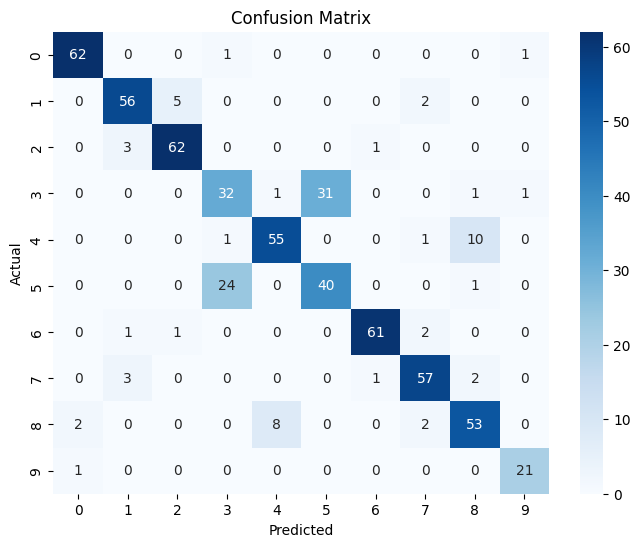
\includegraphics[width=1.\linewidth]{../src/resources/plots/conf-matrix/fe.png}
                  \caption{10 Movements.}
                  \label{fig:cm_all}
                \end{subfigure}%
                \begin{subfigure}{.5\textwidth}
                \centering
                  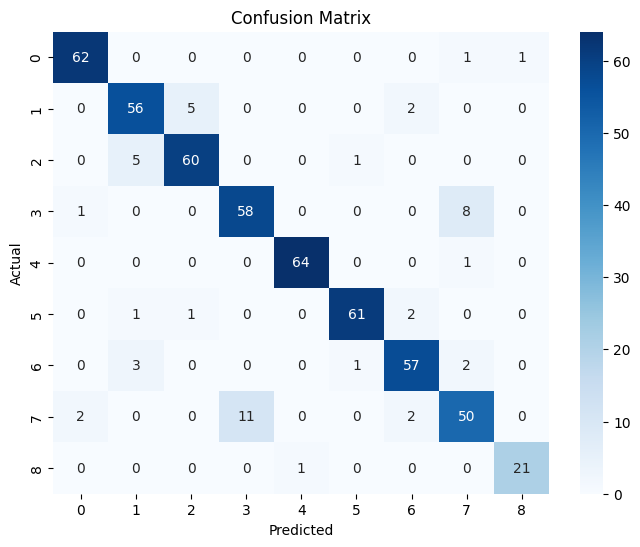
\includegraphics[width=1.\linewidth]{../src/resources/plots/conf-matrix/fe-remove.png}
                  \caption{9 Movements.}
                  \label{fig:cm_remove}
                \end{subfigure}
                \caption{Confusion Matrix of Multi-Layer Perceptron model using Feature Engineering approach.}
            \end{figure}
            
            \newpage

            To confirm this, \textit{3D Visualization} of movements used in Section \ref{sec:movements_visualization} is used. A random sample of \textit{Mat Walk} and \textit{Hoop Walk} is plotted, in Figure \ref{fig: hoop-walk} and Figure \ref{fig: mat-walk} two movements are displayed. They are very similar due to them being both walking movements, the only difference is that in \textit{Mat Walk} patient is walking on a mat while in \textit{Hoop Walk} patient is walking in a hoop. This is the reason why models struggle to differentiate between two movements.

            \begin{figure}[h]
                \begin{subfigure}{.5\textwidth}
                \centering
                  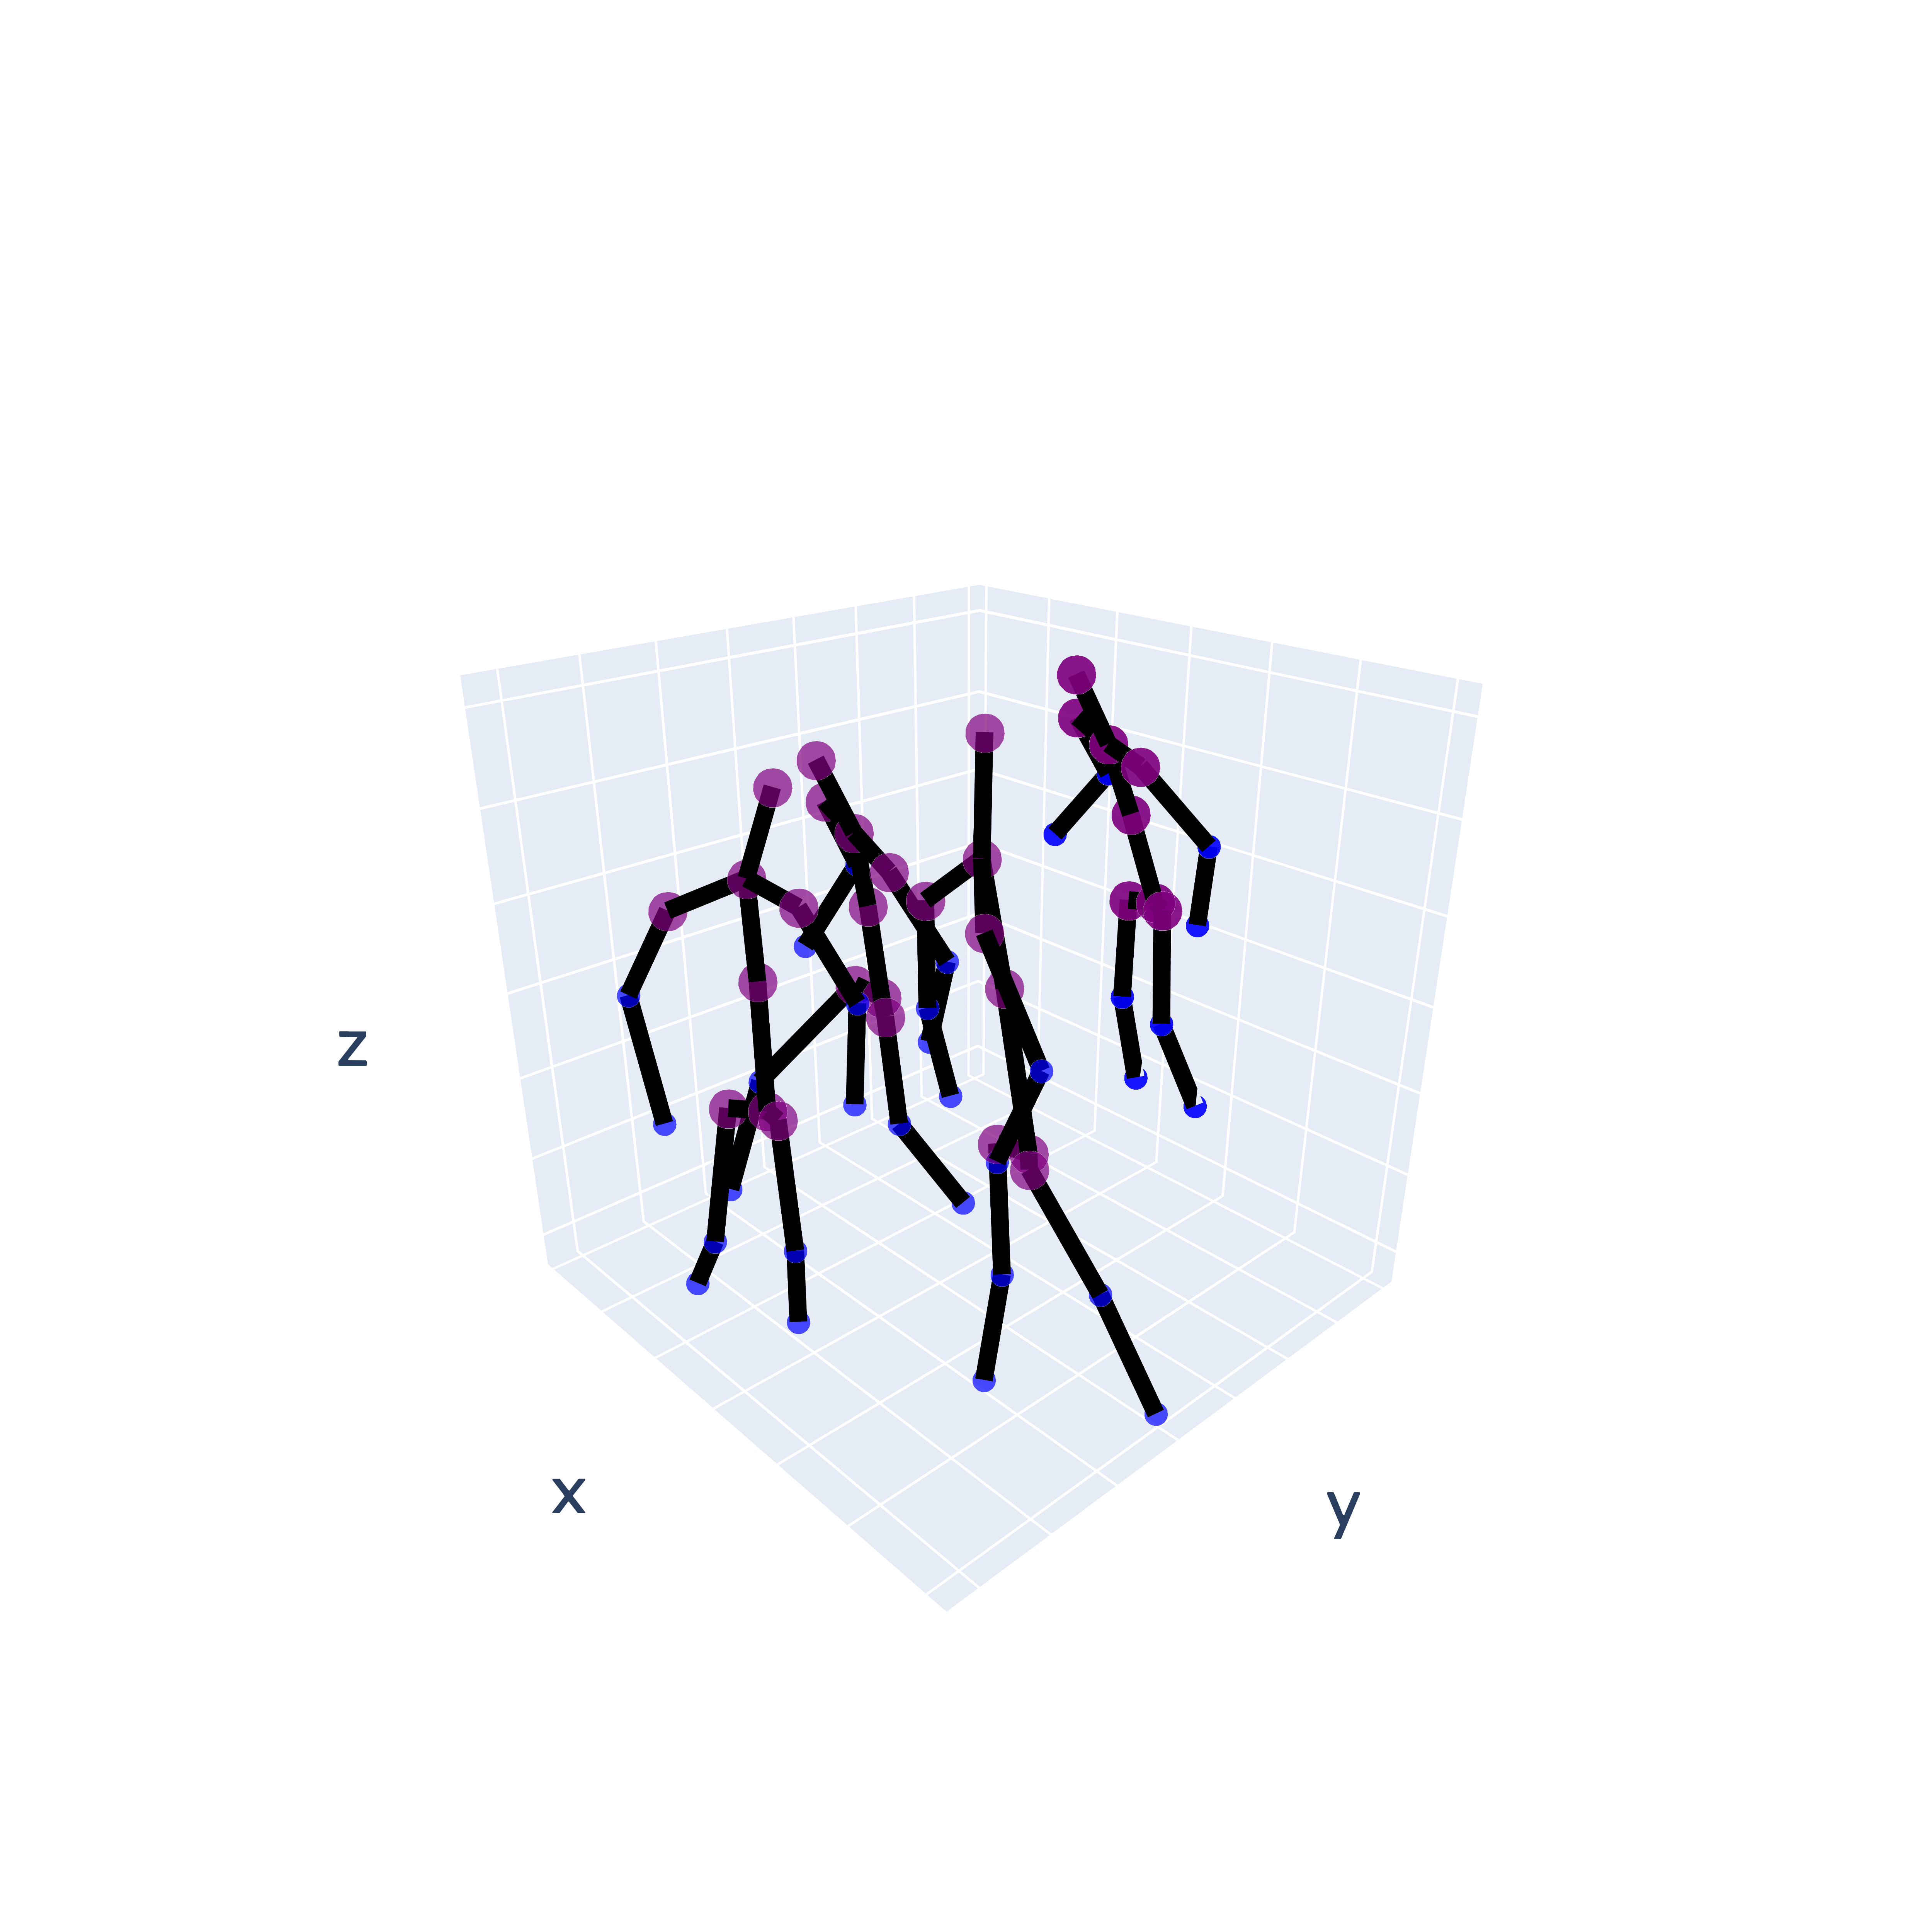
\includegraphics[width=1.\linewidth]{../src/resources/plots/movements/mov-1.png}
                  \caption{Hoop Walk.}
                  \label{fig: hoop-walk}
                \end{subfigure}
                \begin{subfigure}{.5\textwidth}
                \centering
                  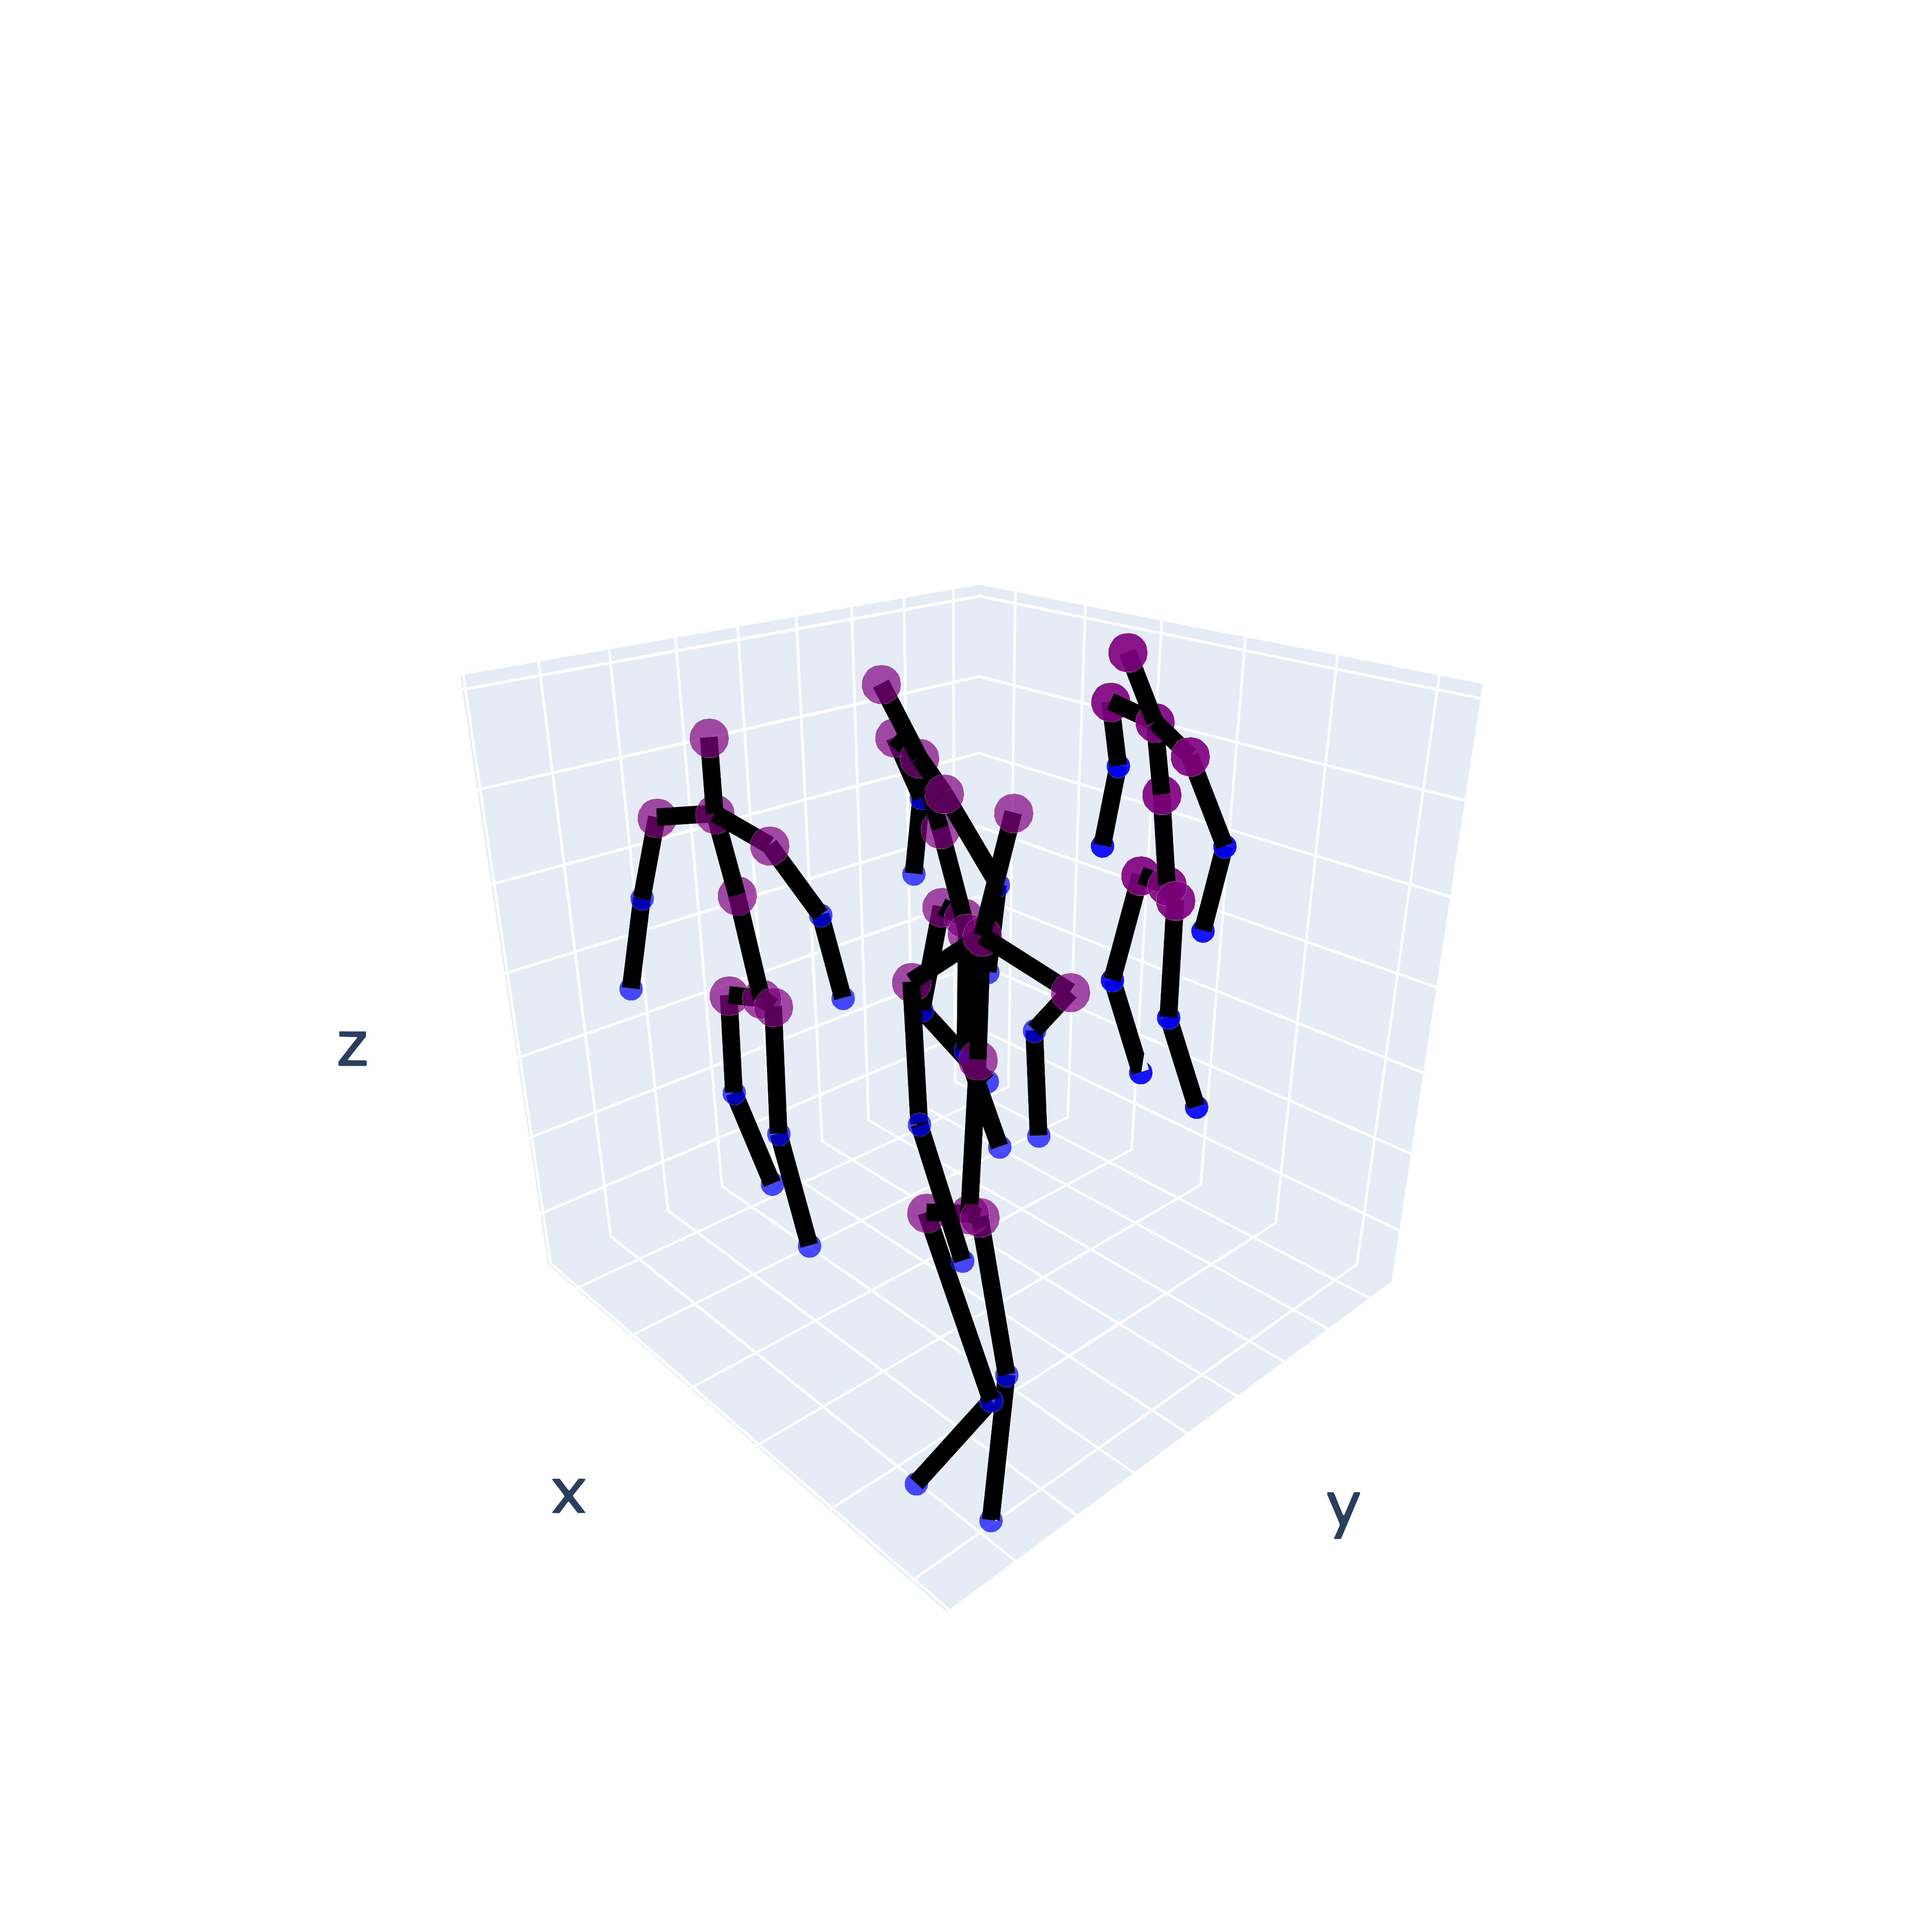
\includegraphics[width=1.\linewidth]{../src/resources/plots/movements/mov-8.png}
                  \caption{Mat Walk.}
                  \label{fig: mat-walk}
                \end{subfigure}
                \caption{3D Visualization plots of two similar movements.}
            \end{figure}

\cleardoublepage


% ================== CHAPTER 5 ==================
\hypersetup{colorlinks=true, linkcolor=blue, citecolor=red}

\chapter{Conclusions} \label{chap:conclusions}

    This chapter presents the key findings of this thesis, highlighting its limitations and reviewing potential approaches for future research to improve results and develop more effective models.

    \section{Discoveries}

        Presented below are the key findings of this thesis: 
        \begin{enumerate}
            \item \textbf{Pre-processed raw data} obtained from the Kinect sensor is suitable for this task of movement classification. However, it alone does not provide enough information for the models to obtain a high accuracy.
            \item \textbf{Feature Engineering} is a crucial process of creating new features from raw data with the goal of improving the accuracy and training time of the models.
            \item \textbf{Multi-Layer Perceptron} is the best-performing model for this task, with a score of \textbf{0.83} using 10 movements and \textbf{0.91} using 9 movements after removing one of the similar movements and using a Feature Engineering approach.
            \item \textbf{Data splitting} techniques are an essential step in the process of training the models, an incorrect split can lead to overfitting and an incorrect evaluation. Using "Patient-ID" as a split criteria is the best approach to avoid any data leakage between training and testing sets.
            \item \textbf{Sequence of frames} is not a good approach to take for this type of data, due to every movement having a variable number of frames, and Machine Learning models need a fixed length input. Transforming data into fixed-length sequences will lead to a loss of information and a decrease in accuracy.
            \item \textbf{3D visualization} of movements allows us to visually identify and label them. It is discovered that "Mat Walk" and "Hoop Walk" are very similar, with the only difference being the object that the patient is walking over. This led to models struggling to differentiate between these two movements and by removing one of them from the dataset accuracy of the models improved.
        \end{enumerate}
    
    \section{Limitations}

        Limitations encountered in this work will be presented, along with an exploration of their impact and the strategies used to overcome them. \\

        A list of 10 movement names was provided with the dataset, however, movements were not labeled according to the list and only a unique ID was assigned to each one. This led to a need to update labels after visually identifying them with the help of a 3D visualization. \\
        While data was collected an unknown number of movements have not been performed correctly by the patients. It was not possible to develop a technique that would identify and remove them, so they have been kept in the dataset. This limitation may have affected the accuracy of the models due to the noise introduced.\\

        The dataset dimensions are relatively small, with only 10 movements and 21 patients. This led to only using Training and Testing sets for the evaluation of the models, as the dataset was too small to split into Training/Validation/Testing sets. A larger dataset is needed to split it into these sets and evaluate the models better. \\
        Features calculated in the Feature Engineering approach are not accurate to the literature due to only using positional data from the Kinect sensor. However, they still provide enough information for models to obtain a high accuracy.

    \section{Future work}      

        Kinect skeleton data is suitable for this task of movement classification, leading to the possibility of implementing new techniques and approaches to improve the accuracy of the models. \\

        Feature Engineering approach obtains a high accuracy and reduces the training time of the models by reducing the dimension of the original dataset. It is recommended to use it if the dataset is going to be scaled up to include more movements and patients, as the training time will increase exponentially.\\
        The number of features has been reduced but it was not possible to tell which ones contribute most to the accuracy of the models. In future work, it is recommended to calculate the importance of each feature and remove the ones that do not contribute to the accuracy of the models. With the help of domain experts, it is possible to calculate new and more meaningful features that can help the models differentiate between movements. \\
        As stated before two movements (Mat Walk and Hoop Walk) are very similar. It is suggested to remove one of them from the dataset to obtain a realistic evaluation of the models, this will help to differentiate between movements that are very similar.\\
        
        This thesis only used Machine Learning models from \textit{Scikit-Learn} library. It is possible to implement new models from \textit{TensorFlow} library, such as \textit{Convolutional Neural Networks} and \textit{Long-Short Term Memory} networks. These models are more complex and require a larger dataset to train on, but they can obtain a higher accuracy than models used in this thesis with a correct implementation. \\
        It is crucial to acquire new data from the Kinect sensor and add new movements and patients. This will allow us to scale up the dataset and study how models perform on more classes and patients. \\

        The possible approaches for future work on this task are endless, above are only a few suggestions that can be implemented. The goal of this thesis is to study the feasibility of using Kinect skeleton data for movement classification and provide a baseline for future research with this type of data. \\
    
    \cleardoublepage



% ================== ACKNOWLEDGMENTS ==================
%\chapter*{Acknowledgements}
    \addcontentsline{toc}{chapter}{Acknowledgements}
    \begin{large}
    %* My advisor
    I would like to thank my advisor Prof. \textbf{Maurizio Mancini}.
   
    \vspace{2mm} 
    % My Family
    \noindent I am extremely grateful to my mother \textbf{Rodica} and my father \textbf{Dorin} for leaving their 
    country, their family and friends behind to give me a better future.
    Words cannot express my gratitude for their support and love throughout my life. 

    \vspace{2mm}
    %* My partner 
    \noindent I would like to thank my girlfriend, \textbf{Margherita}, for her support and patience during my whole university 
    experience. We met a few weeks before we both started our university journey and we have been toghether 
    ever since, and i am glad to have shared this experience with her. I was able to learn a lot from her 
    and i am grateful for that.

    \vspace{2mm}    
    % Mimmi and Shelby 
    \noindent I am also thankful to my two cats \textbf{Mimmi} and \textbf{Shelby}, they 
    have been with me during my sleepless nights even tough most of the time the were sleeping right 
    next to me.
    
    \vspace{2mm} 
    %* My colleagues
    \noindent Lastly, I would be remiss in not mentioning my colleagues. I started this journey with a small group 
    of people Mattia, Edoardo and Michael and i am glad to have met them and shared this painfull but also 
    rewarding experience with them. I would also like to thank all the other people that i met during these 
    years.
    

    \end{large}

\backmatter
\phantomsection

% ================== BIBLIOGRAPHY ==================
\addcontentsline{toc}{chapter}{Bibliography}
\bibliographystyle{sapthesis}
\bibliography{/Users/lucian/GitHub/Thesis/Thesis/src/references.bib}


%! ================== Temp stuff ==================
% \begin{lstlisting}
%     # Comment test
%     def my_range(start, end, step):
%         while start <= end:
%             start += step

%     for x in my_range(1, 10, 0.5):
%         print('Hello World!')
% \end{lstlisting}

\end{document}